\section{Gestión de Tareas}
        El usuario tiene a su disposición 2 funciones para la gestion de tareas:
        \subsection{Consultar Tareas}

            Si el usuario da clic a la opción del menú \textit{Ver Tareas}, se le redirecciona a la siguiente pantalla:
            \begin{figure}[H]
                \centering
                \hypertarget{asignart}{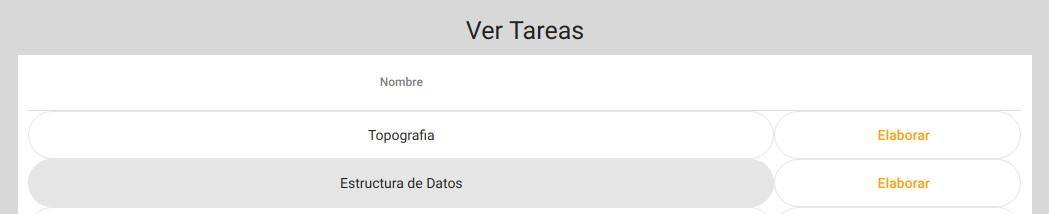
\includegraphics[width=0.7\linewidth]{images/Tareas/Vertareas}}
                \caption{Tabla de tareas}
                \label{asignart}
            \end{figure}
            Donde el usuario ve una tabla con todas las tareas relacionadas con él.

        \subsection{Asignar Tareas}

            Para ello, el usuario da clic en el botón con el icono de una tablita que esta en la fila de la Unidad de Aprendizaje a la que esta asociada la tarea.

            \begin{figure}[H]
                \centering
                \hypertarget{boton}{
\includegraphics[width=0.7\linewidth]{images/Tareas/boton}}
                \caption{Botón Asignar}
                \label{boton}
            \end{figure}

            Al hacer esto, el sistema redireccionará al usuario a la pantalla siguiente donde puede seleccionar un usuario para asignarle una tarea.

            \begin{figure}[H]
                \centering
                \hypertarget{asigna}{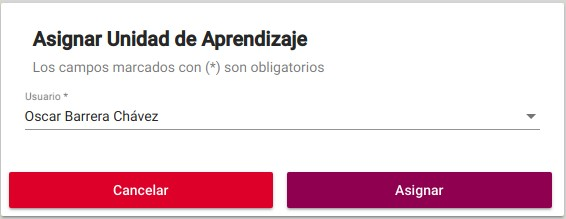
\includegraphics[width=0.7\linewidth]{images/Tareas/Asignando}}
                \caption{Seleccion de usuario para tarea}
                \label{asigna}
            \end{figure}

           Cuando da click en el boton \IUbutton{Asignar} y aparece el siguiente mensaje:
            \begin{figure}[H]
                \centering
                \hypertarget{asignar}{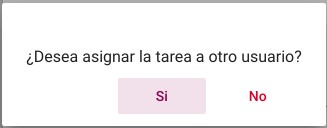
\includegraphics[width=0.7\linewidth]{images/Tareas/Asignarotro}}
                \caption{Seleccion de otro usuario}
                \label{asignar}
            \end{figure}
            Esto permite asignar una tarea a varios usuarios.



